%!TEX root = FreeRtos ARM uController.tex


\subsection{Echtzeitsysteme und Echtzeitbetriebssysteme}
\label{sec:Echtzeitsysteme}
Mit der steigenden Leis\-tungs\-fähig\-keit von modernen $\mu$\-Pro\-zesso\-ren, steigen auch die Anforderungen an die Software die auf diese Systeme aufsetzt. Viele dieser Systeme fordern trotz ihrer Komplexität, dass Teile des Pro\-gramm\-ab\-laufs in bestimmten zeitlichen Grenzen ausgeführt werden und somit vorhersehbar und deterministisch sind. Systeme die solchen Anforderungen unterliegen werden Echtzeitsysteme genannt. Bezogen auf ihre Zuverlässigkeit unterliegen Echtzeitsysteme einer weiteren Unterteilung, in Echtzeitsysteme mit weicher Echtzeitanforderung (soft realtime systems) und Echtzeitsysteme mit harter Echtzeitanforderung (hard realtime systems). Ein weiches Echtzeitsystem soll eine Aufgabe in den vorgegebenen zeitlichen Grenzen ausführen. Ein Über\-schreiten der zeitlichen Grenzen ist grundsätzlich nicht erlaubt, führt aber nicht unmittelbar zu einem Fehler oder einem Versagen des Gesamtsystems. Ein hartes Echtzeitsystem hingegen muss die gestellte Aufgabe in den vorgegebenen Grenzen aus\-füh\-ren. Durch eine Überschreitung wird das System unbrauchbar und führt dazu, dass das System nicht im vorgesehenen Szenario eingesetzt werden kann. Dabei ist ausdrücklich zu beachten, dass Echtzeit nicht bedeutet, dass ein Programm besonders schnell ausgeführt wird. Die Ausführung eines Programms kann beispielsweise auch gewollt langsam sein und gerade deshalb den gestellten Echtzeitanforderung genügen. Einige Beispielsysteme und deren Echtzeitzuordnung wird in Tabelle \ref{tab:BeispieleEchtzeitsystem} gezeigt. 
\begin{table*}
\centering
	\begin{tabular}{|l|l|l|}
		\hline
		\textbf{Beispiel} & \textbf{Echtzeit Typ}  & \textbf{Auswirkung} \\
		\hline
		Tastatur Controller & Soft Realtime & Kurzfristig verzögerte Ausgabe \\
		\hline
		Echtzeit Media Streaming  & Soft Realtime & Bild und Ton kurzfristig asynchron \\
		\hline
		Computer Numerical Control (CNC)  & Hard Realtime & Fehler bei der Fertigung des Teils\\
		\hline
		Airbag System  & Hard Realtime & Möglicher Personenschaden\\
		\hline
	\end{tabular}
	\caption{Beispiele von Echtzeitsystemen und deren Auswirkung beim über- oder unterschreiten der Anforderungsgrenzen}
	\label{tab:BeispieleEchtzeitsystem}
\end{table*}
Um die grund\-sätz\-liche Funktionalität eines Echtzeitbetriebssystems zu erläutern, werden zuerst die Grundmodelle für den Programmablauf eingebetteter Systeme beschrieben. Der Programmablauf lässt sich auf drei Modelle zu\-rück\-füh\-ren (Abbildung \ref{fig:Programmablauf}). 
\begin{figure}[ht]
	\centering
		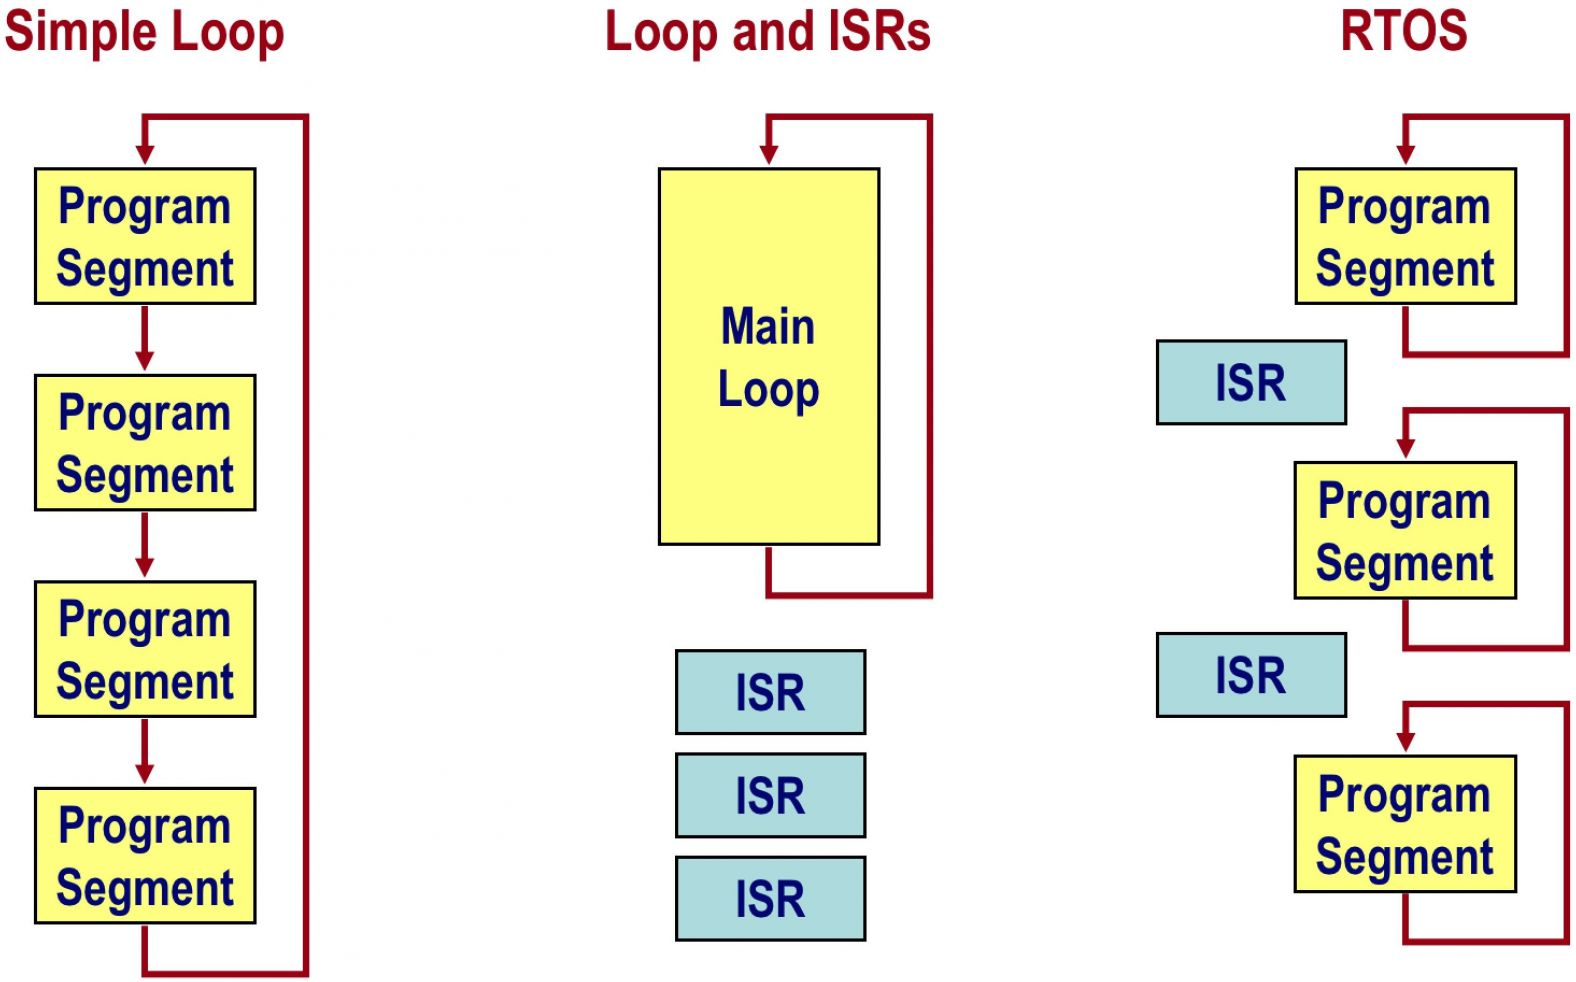
\includegraphics[width=0.3\textwidth]{Pictures/EmbeddedCom/cwrtos2f5c.jpg}
	\caption{Übersicht Programmabläufe in embedded Anwendungen. Unterscheidung von zwei Hauptkategorien: Schleifen-gesteurte Anwendungen und Event-gesteurte Anwendungen. Bild-Quelle~\protect\citeA{RTOSRevealed}}
	\label{fig:Programmablauf}
\end{figure}
Eingebettete Anwendungen können in einer einzigen Schleife (mit oder ohne Interrupt Unterbrechungen) laufen oder aber in event-gesteuerten ne\-ben\-läuf\-igen ei\-gen\-stän\-dig\-en Pro\-gramm\-ab\-schnit\-ten (Thre\-ad oder Task\footnote{Nachfolgenden wird Task benutzt, da dies der geläufige Begriff bei FreeRTOS ist. In der Literatur zu Echtzeitsystemen ist der Begriff nicht exakt definiert.}) ausgeführt werden. Die ne\-ben\-läuf\-ige Aus\-füh\-rung der unterschiedlichen Programmsegmente ist nur durch einen Scheduler, welcher Teil eines RTOS Kernels ist, zu erreichen. Ein RTOS Kernel abstrahiert von der zugrunde liegenden Hardware und ermöglicht weitergehende Steuerung, beispielsweise durch Verwaltung von Timing Informationen. Der Kernel stellt durch den Scheduler sicher, dass die näch\-ste Task rechtzeitig ausgeführt wird. Der Entwickler ist dafür verantwortlich, dass die Task die ge\-wün\-schte Aufgabe im zeitlichen Rahmen ausführt. Durch den Einsatz des RTOS Kernels kann der Entwickler jedoch auf Spezifika der Hardware verzichten und die Funktionen des Kernels verwenden. Wie sichergestellt werden kann, dass eine Task harten oder weichen Echtzeitanforderungen entspricht, wird Abschnitt \ref{sec:Echtzeitanalyse} beschrieben. Für viele kleine Anwendungen kann die Nutzung einer einzigen Schleife durchaus sinnvoll sein, wenn beispielsweise die Ressourcen so knapp sind, dass ein Overhead durch zusätzliche Verwaltungsfunktionen ausgeschlossen werden muss. Ein großer Nachteil der "`einschleifen Variante"' ist die permanente Nutzung des Prozessors, auch "`processor hogging"' oder "`CPU hogging"' genannt. Um den Prozessor in dieser Variante in einen Energiesparmodus zu versetzen sind umfangreiche Kenntnisse über den Prozessor sowie eine sehr strukturierte Programmierung erforderlich, die gerade bei Anpassungen der Software zu Problemen führen kann. Besonders bei akkubetriebenen Geräten wie IoT Devices oder Mobiltelefonen wird sehr genau auf die Energieaufnahme geachtet. Ein RTOS Kernels hingegen arbeiten mit einem Event gesteuerten Programmablauf, ein "`CPU hogging"' kann somit vermieden werden. Des Weiteren bieten viele RTOS Kernel sehr einfache Lösungen zur effektiven Nutzung von Energiesparmodis. Dies wird in Abschnitt \ref{sec:Low Power Modes} am Beispiel von FreeRTOS und einem ARM $\mu$Prozessor demonstriert. Neben der Echt\-zeit\-fähig\-keit gibt es aber noch viele weitere Vorzüge für den Einsatz eines Echtzeitbetriebssystems. Durch das Herunterbrechen der Anwendungen in Tasks entstehen viele kleine Module, die jeweils eine kleine Teilaufgabe des Gesamtsystems über\-neh\-men. Durch ein sauber definiertes Interface zur Kommunikation der Tasks, lässt sich die Entwicklungsarbeit leicht auf mehrere Teams verteilen. Dies ermöglicht auch den Einsatz von agilen Entwicklungsmethoden wie Scrum in der Entwicklung von eingebetteten Systemen. Ein weiterer großer Vorteil ist die Erweiterbarkeit von RTOS Anwendungen. Bei Änderungen von Anwendungen die in einer Schleife laufen, ist oft der gesamte Code von dieser Änderungen betroffen. Ein RTOS hat durch die Interprozesskommunikation eine natürliche Lose-Kopplung zwischen den einzelnen Programmfunktionalitäten. Das Än\-dern oder Hinzufügen von Tasks ist somit wesentlich einfacher, da andere Tasks nicht unmittelbar durch diese Än\-der\-ung betroffen sind. 




